%---------------------------------------------------------------------
% This file provides a skeleton UCL DIS CDT report.
% \pdfinclusioncopyfonts=1
% This command may be needed in order to get \ell in PDF plots to appear. Found in
% https://tex.stackexchange.com/questions/322010/pdflatex-glyph-undefined-symbols-disappear-from-included-pdf
%---------------------------------------------------------------------
% Specify where LaTeX style files can be found.
\newcommand*{\DISCDTLATEXPATH}{latex/}
% Use this variant if the files are in a central location, e.g. $HOME/texmf.
%---------------------------------------------------------------------

\documentclass[NOTE, disdraft=true, UKenglish]{\DISCDTLATEXPATH UCLCDTDISdoc}
% The language of the document must be set: usually UKenglish or USenglish.
% british and american also work!
% Commonly used options:
%  cdtdraft=true|false   This document is a UCL CDT DIS draft.
%  paper=a4|letter       Set paper size to A4 (default) or letter.

%--------------------------------------------------------------------- 
% Add you own definitions here (file dis-gp-defs.sty).
%\usepackage{dis-gp-defs}
%---------------------------------------------------------------------


%--------------------------------------------------------------------- 
% Files with references for use with biblatex.
% Note that biber gives an error if it finds empty bib files.
\usepackage{biblatex} % uncomment if use addbibresource command
\addbibresource{template/PNET_project.bib}
%--------------------------------------------------------------------- 

% Paths for figures - do not forget the / at the end of the directory name.
\graphicspath{{logos/}{figures/}}


%---------------------------------------------------------------------
% Generic document information
%---------------------------------------------------------------------
% Title, abstract and document 
%-------------------------------------------------------------------------
% This file contains the title, author and abstract.
% It also contains all relevant document numbers if needed.
%-------------------------------------------------------------------------

% Partner Logo
% put the name of the logo image file found in graphics path
\DISPartnerLogo{logos/UCL_purple.png}


% Title
\DISTitle{Improving radiosensitivity predictions of brain cells using a biologically informed neural network}

% Draft version:
% If given, adds draft version on front page, a 'DRAFT' box on top of each other page, 
% and line numbers.
% Comment or remove in final version.
\DISVersion{0}

% Abstract - % directly after { is important for correct indentation
\DISAbstract{%
  One of the current most effective treatments for brain tumor's is radiotherapy. However, this has the side-effect of damaging healthy cells with potentially severe consequences. Improvements in radiotherapy treatment such as proton therapy allow a more spatially localized treatment. However, the sensitivity of different cell types to radioactivity is not currently well modeled. We present a method for predicting the radio-sensitivity of a cell based on its genetic content using a biologically informed neural network. We compare the use of different data features for training this model, different network architecture and develop a procedure for transfer learning, where drug response data is incorporated into the model training. We compare the model performance using a cross-validation procedure ensuring unbiased performance estimates with faithful uncertainty estimates. We find ...
}


% Authors and list of contributors to the analysis
\usepackage{authblk}
\author[a]{Toby Dixon}
\author[a]{Dakshesh Kololgi}
\author[b]{Jason Ran}

\affil[a]{University College London}


% DIS reference code if ever used
\DISRefCode{UCLCDTDIS-2024-XX}

% Author and title for the PDF file
\hypersetup{pdftitle={UCL CDT DIS Document},pdfauthor={The UCL CDT DIS}}

%---------------------------------------------------------------------
% Content
%---------------------------------------------------------------------
\begin{document}

\maketitle

\tableofcontents

\clearpage


%---------------------------------------------------------------------
\newpage
%---------------------------------------------------------------------

\newpage
%---------------------------------------------------------------------
\section{Introduction}
\label{sec:introduction}
Cancer is one of the largest causes of mortality, leading to intensive research into cancer treatments. One of the most promising is radiotherapy, contributing to $\sim$40\% of treatments. In this treatment, malignant tumours are treated with ionising radiation (typically X-rays) that form free radicals that may cause tissue damage and secondary cancers. 

To recognise the benefits and limitations of modern radiotherapy, it is important to understand some fundamentals of cell biology. The behaviour of human cells are largely determined by their DNA (deoxyribonucleic acid) which encode the nature of the complex interactions and pathways that take place in the cell. Starting from a single human cell, the DNA contains the information needed to develop into a complex organism, and therefore all the cells in a human contain the same DNA. DNA molecules have double helix structures, forming chains from sequences of 4 basic units (nucleotide), A, C, G, and T, with length on the order of 3 billion nucleotide pairs. Each DNA molecule can be organised into a series of $\sim$25000 genes, each of which can be seen as a different section of the DNA molecule \cite{genetics_basics}. The particular composition of each gene encodes the processes and proteins associated with it, and the \textit{gene expressions} within a cell allows it to have different functions, thereby determining it's \textit{phenotype}. Therefore cells of different organs will contain identical DNA, with differing gene expressions that allow different functions. Basic cell functions also require DNA to interact closely with RNA (ribonucleic acid), which transcribe genetic data from genes to protein synthesis sites, and plays important roles in RNA editing and gene expression regulation. \cite{RNA} The study of the constituent components and processes in cells, especially their 3 dimensional structures, is a broad and highly active area of research. There are many in-depth and extensive reviews of this available.

Radiotherapy works by causing DNA damage to tumour cells as an effective treatment to destroy tumour cells or stop cell proliferation. However, these treatments still induce a significant amount of damage to healthy cells which can have severe side effects, as the physical effects of radiation are independent of cell type \cite{rev_radio}. Furthermore, the complex pathways induced by DNA damage are not fully understood, and strongly depend on the genetic structure of the patient. For instance, it is possible that DNA damage can lead to downstream effects that promote cell proliferation or have effect DNA repair mechanisms, both of which increase radio-resistance. Therefore, developing methods to predict cell radiosensitivity would enable more optimal radiotherapy based on genetic sequences, that would maximise damage to tumour cells while minimising other side effects, or guiding treatments where radiotherapy may not be suitable at all \cite{rev_radio}.  Developments in radiotherapy such as proton beam therapy \cite{proton_beam} allow for more spatially targeted treatments, which can be optimised for each patient and diagnosis. This opens up the possibility of optimising treatments to avoid regions expected to have high radiation sensitivity.  Accurate predictions of cell radio-sensitivity could revolutionise treatments allowing for a personalised treatment based on a patients individual genetic sequence similar to some chemotherapy treatments \cite{breast_cancer}.

\\ \indent 
Previous efforts to predict radio-sensitivity based on genetic data have been investigated using some classical approaches such as least squares regression \cite{rev_radio,SCOTT2017202}. 
However, advancements in gene sequencing technology and the availability of computational resources have staged genomics as an ideal problem for machine learning and artificial intelligence (AI) \cite{review}, which has developed into a cornerstone of bioinformatics. In particular, \textit{Deep Learning} has the ability to create highly non-linear models which can make use of large feature spaces, which makes it a leading predictive model in genomics for accuracy, especially for \textit{sequence - to - activity} models that predict the outcome of a process based on the genetic sequence. 

\\ \indent Unsurprisingly machine learning methods have been applied to radio sensitivity predictions (see for example\cite{speers2015development}). However, these methods generally require heavy regularisation due to the small available datasets. The large number of parameters also causes the model to be susceptible to over-fitting on the small available omics datasets. An emerging interest in such Deep Learning research has been model explainability, as these models are able to learn millions of model parameters to form predictions with none to little insight into how the prediction is made. As previously discuss, this causes a problem in medical fields where often the understanding the causes and effects of processes are equally important, as the ultimate goal is to find reliable biomarkers that can explain radiosensitivity. This problem is exacerbated by low data settings which can easily lead to over-fitting. At the current time, a lack of cells with both genetic and radiation sensitivity data available presents this exact issue. 

\\ \indent  In this work we attempt to improve on this by developing a radio-sensitivity predictor using a biologically informed neural network (BNN) \cite{review,review_2}. This type of model consists of a sparse neural network where the network connections represent known biological processes, which are compiled in genetic databases \cite{reactome,go_1,go_2}. This has the advantage that the number of fitted parameters is much smaller, preventing over-fitting and the outputs of the model become more interpretable, potentially leading to biological insights.

\\ \indent As previously mentioned, this work uses genomic data as predictors. There are various sources of cancer cells with genetic data used in medical research. These include patient-derived tumour xenografts (PDXs) - created by growing human tumour tissue in immunodeficient animal hosts \cite{PDX}, which allows some physiological processes to take place when investigating human tumour cells. Another pre-clinical setting for human cell research is from \textit{cell lines}, which are human-derived cells inhabited in vitro cell populations. Cell lines have the advantage of being cost-effective, providing a basis for reproducible results, and sidesteps ethical concerns of human/animal tests. We focus on 3 genetic features; gene expression, copy number violation, and mutations.  Gene expression is a measure of the transcription of the DNA sequence into RNA.
Copy number variation represents the repetition of certain sequences in the DNA or RNA \cite{CNV}. These genetic features are expected to be related to processes of radiation damage \cite{rev_radio} and could be used to predict radiation sensitivity.

\\ \indent 
The model we used is known as P-NET\cite{elmarakeby_biologically_2021}, developed for the classification of prostate cancer cells, which has since been adapted for radio-sensitivity predictions by the UCL Medical Physics and Biomedical Engineering department\cite{cosmin_thesis}. P-NET is a BNN with connections based on the Reactome network \cite{reactome} which contains a hierarchical network of biological pathways relevant to tumour cell treatment. The Reactome network is then used to inform the connections between the nodes of the neural network, with the input layer corresponding to the gene sequence. However, owing to the complex nature and signalling involved in biological processes, there exists many such onotlogies that organises this information which have been used in various other studies \cite{drug_cell}. The novelty of our work lies in using a separate hierarchy (leading to a separate network architecture), \textit{Gene Ontology} \cite{go_1, go_2}, to inform the biological aspects of P-NET and investigate any possible improvements. In this work we develop a procedure for systematic tuning of the parameters of this radiosensitivity model and develop a procedure for unbiased and statistical comparisons of different models.

In addition, we have explored applying \textit{transfer learning} \cite{McEwan} to radio-sensitivity predictions. Transfer learning is a common pipeline of ML model training that aims to make use of low - level similarities between datasets of related fields. Transfer learning (and extensions such as metalearning \cite{MAML} and multitask learning \cite{multitask}) have been successfully applied in bioinformatics research, such as predictions of drug response in clinical settings based on genetic sequencing from in-vitro cell line data. In the P-NET setting, we hypothesise that similarities between the underlying mechanisms of action used in drug and radiation treatments. If this is true, we can develop a novel method of radio-sensitivity prediction using data from extensive drug response datasets to supplement the radiation responses.

\\ \indent 
This report describes a systematic comparison of P-NET BNN used for cell line radio-sensitivity predictions using different data types, network architectures and transfer learning based methods. 
In \ref{sec:data} we describe the collation of genetic data used for this study, in \ref{sec:method} we provide a more detailed description of the P-NET model and our framework for model comparisons. Finally, in section \ref{sec:results} we describe the results. The outlook for future studies is described in \ref{sec:Discussion}.
 


\section{Methods}
\label{sec:method}
For this work, we employ a biologically informed neural network to predict the radio-sensitivity. This is based on our adaptation of P-NET \cite{cosmin_thesis}. A typical dense neural network has millions of connections, and thus weights to tune. This can easily lead to over-fitting where the model predicts well on the training dataset but not on unseen data. A solution to this is to encode some prior knowledge into the model's architecture. In this way, we create a sparse network where the connections represent known biological pathways. In our work this is done using P-NET \cite{elmarakeby_biologically_2021} considering prior biological information from two databases Reactome \cite{reactome} and Gene Ontology \cite{go_1,go_2}.

Biologically informed neural networks emerged analogously to physics-informed neural networks which utilised partial differential equations to constrain the number of free parameters, leveraging the symmetry of physical systems.  

\subsection{Data}
\label{sec:data}


\begin{figure}
    \centering
    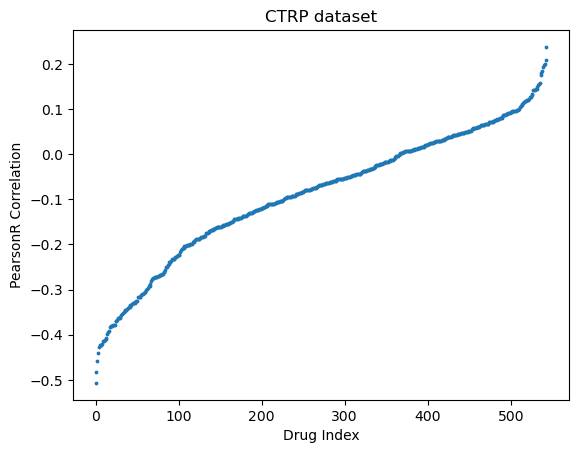
\includegraphics[width=9cm]{Figures/CTRP_correlation.png}
    \caption{CTRP correlation}
    \label{CTRP correlation}
\end{figure}
%We use data from the Cancer Cell Line Encyclopedia (CCLE) dataset \cite{ccle}.

\\ \indent 
This work is focused on the Cleveland dataset, which characterises radiation response (measured by a dose-response curve - AUC) of 511 cancer cell lines and provides genetic for each cell line \cite{manem}. All cell lines found in Cleveland can also be the Cancer Cell Line Encyclopaedia Project (CCLE) \cite{yard}, which is a collaboration between the Broad and Novartis Institutes. CCLE aims to provide drug responses (also measured in dose-response curves -AAC) of cancer cell lines with detailed genetic characterisation that can be used in bioinformatic studies. 

In addition to CCLE, we also look at the CTRPv2 \cite{CTRP} dataset. Similar to CCLE, CTRPv2 provides the drug response of cell lines, with 968 drugs and 8338 cell lines contained in the dataset. In total, CCLE contains genetic data for 1094 cell lines, and studies 14 drugs. However, it should be noted that not all drugs are tested on cell lines (i.e. there are less than $1094\times14 = 15316$ data points). Unfortunately, CTRPv2 does not provide genetic data, so only overlapping cell lines between CCLE and CTRPv2 can be used in our study for radio-sensitivity prediction. The Cleveland dataset has been curated in the RadioGX package \cite{manem}, while CTRPv2 and CCLE can both be found in PharmacoGX \cite{pharmaco}. These R packages are designed to provide easy-to-use sources of standardised data.

\\ \indent We consider the gene expression, copy number variation (CNV) and mutations data. We preprocess the CNV data to consider separately amplification's and deletions of a sequence. In each case the data is a binary number representing whether a sequence has the normal copy number or not.

For each drug in CCLE and CTRPv2, intersecting cell lines between the Cleveland dataset and CCLE/CTRPv2 were taken, and a PearsonR correlation coefficient was calculated for each drug in order to determine suitable drugs. For drugs in both CCLE and CTRPv2 datasets, a union of cell lines were taken prior to the intersecting with the Cleveland dataset. An example plot of the ordered PearsonR correlation coefficients for the CTRPv2 drug responses is shown in Figure \ref{CTRP correlation}. As drug-sensitivity and radiation-sensitivity are described using AAC and AUC respectively, negative correlations correspond to higher similarity of cell response. Of the best correlating drugs, drugs with at least 300 cell lines with genetic data contained in the CCLE dataset formed a list of 10 drugs used for transfer learning.




\subsection{Network architecture}

Fundamentally, neural networks are regression and classification tools inspired by the human brain. Human brain cells, called neurons, form a complex and highly interconnected network and send electrical signals to each other to help humans process information. Similarly, an artificial neural network is made of artificial neurons that are arranged in layers to work together and solve problems. A simple example is shown in figure \ref{fig:basicNN}. From the left, we have an input layer that allows for inputs of observables from the outside world. Then, for a dense network, each input node or neuron is connected to every node in a subsequent hidden layer. Neural networks can have a large number of hidden layers and each hidden layer analyses the output of the previous layer, processes it, and passes it onto the next layer. Finally, the output layer gives a final result of all the data processing by the artificial neural network, it can have multiple or single nodes, depending on the problem, in this example, most people's gender can be simplified to a binary, male or female and so only one output node is required to classify an individual, given their height and weight according to their gender. Multi-class classification problems and regression problems might require multiple output nodes. In some scientific applications, two output nodes may be needed, one to provide the measurement and the other for the measurement uncertainty. Deep neural networks have several hidden layers sometimes with millions of nodes linked together that facilitate the representation of very complex problems. P-NET falls under a deep neural network category due to its multiple hidden layers. 

Figure \ref{fig:basicNN}, also displays edges which represent a weighting of the connections between neurons in different layers, although weights are usually adjusted in the training process, some are hard-coded in P-NET and are used to represent biological processes more efficiently than a fully connected network. Neural network training is the process of teaching a neural network to map between input and output so that it can perform a task. Training involves using training data to continuously adjust the weights of the edges between the layers of a neural network until an optimal level of representation has been reached. The mean squared error or loss (MSE, equation \ref{eq:mse}) is the main way we quantify the performance of a neural network, training data, $\textbf{x}$, is inputted into the network and the network's output is assessed using MSE. The loss is then minimised over successive iterations by adjusting the weights \cite{noauthor_what_nodate}. 

\begin{equation}
    MSE = \frac{1}{n} \sum_{i=1}^{n} (y_{true} - y_{pred})^{2}
    \label{eq:mse}
\end{equation}

Stochastic gradient descent \cite{noauthor_what_nodate, elmarakeby_biologically_2021} tells us how to change the network's weights and biases to minimise the loss and it is the method used by P-NET while training. During the training process, another set of data, unseen by the neural network called the validation set is used to check that the neural network is not overfitting the training data. The validation set is not used to change the weights of the network. Once training and validation are complete, the network is then fed test data that predicts outputs based on the trained weights. P-NET's goal is to use this methodology to predict the radiation sensitivity of cancer cell types based on gene expression data and radiation data.

There are multiple different types of neural networks \cite{noauthor_what_nodate}, and the feed-forward variant, which is the type that P-NET is, involves processing data in one direction, from the input node to the output node. Feedforward networks use the training process to improve predictions over several training iterations. This is in contrast with backpropagation networks and convolutional neural networks

\begin{figure}
    \centering
    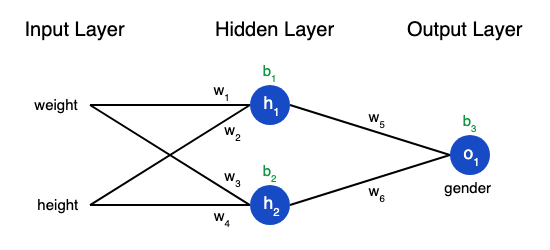
\includegraphics[width=\linewidth]{Figures/basicNN2.png}
    \caption{A simple neural network relating two features, height and weight, with an output, gender. The image was obtained from \cite{noauthor_machine_nodate}}
    \label{fig:basicNN}
\end{figure}

P-NET was originally developed to classify prostate cancer tumours into either primary or metastatic types. P-NET consists of six layers arranged such that the constituent neurons encode the hierarchical manner of the Reactome or Gene Ontology bio-informatics databases. Each successive layer encodes increasingly more complex biological processes. This was implemented by selectively connecting neurons between layers depending on the hierarchies in Reactome or Gene Ontology.

This work significantly re-structured P-NET to enable connections between layers to be informed by Gene Ontology in addition to Reactome. We draw from Kuenzi et al.'s implementation of the DrugCell Deep Learning model that, in analogy with P-NET, utilises Gene Ontology for cancer cell drug sensitivity prediction \cite{kuenzi_predicting_2020}.

\begin{figure}
    \centering
    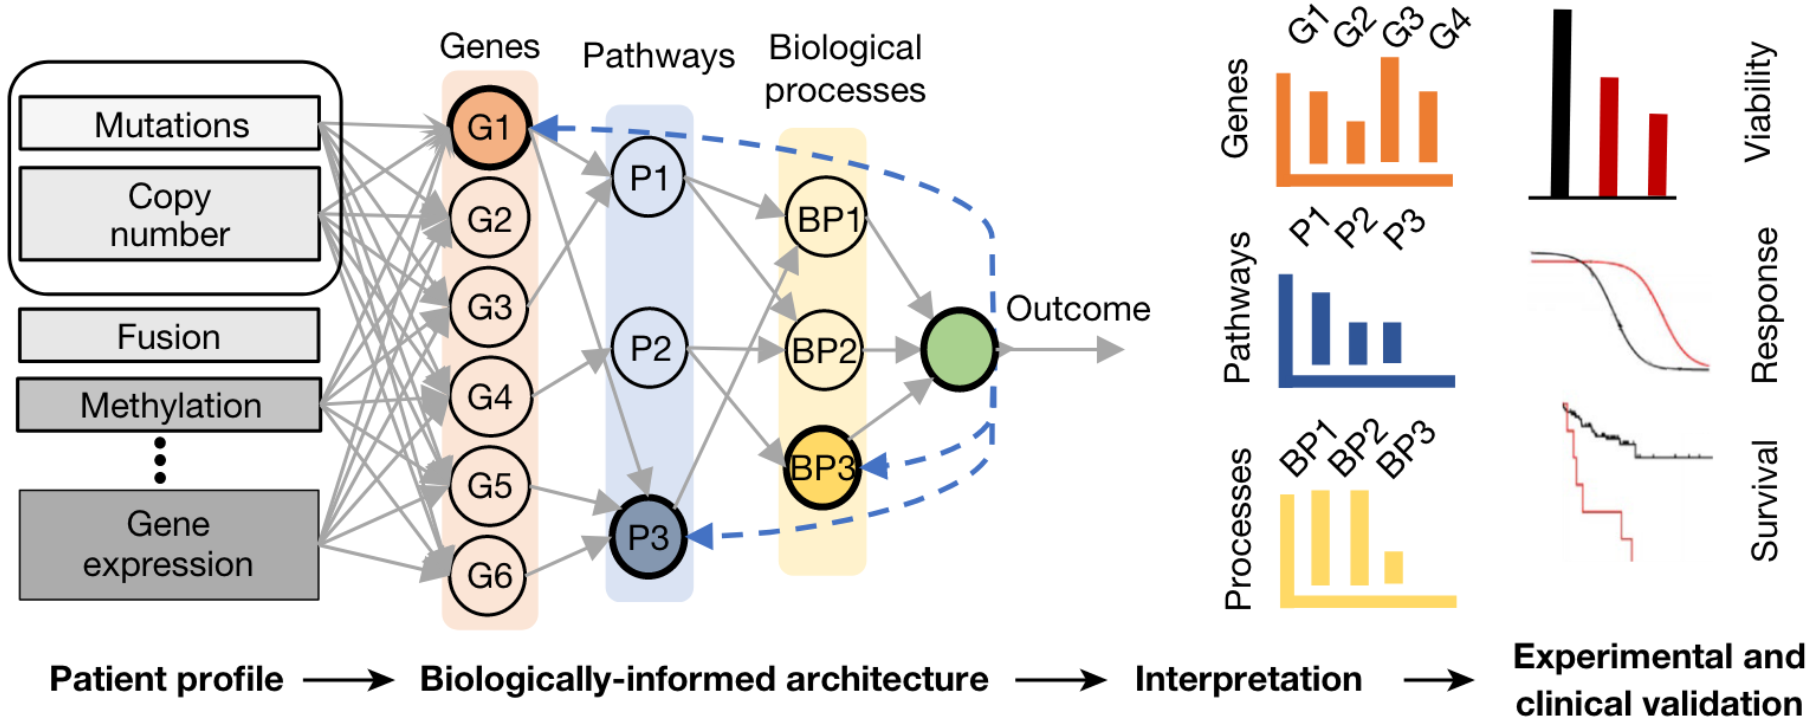
\includegraphics[width=\linewidth]{Figures/pnet_architecture.png}
    \caption{Architecture of the original P-NET neural network \cite{elmarakeby_biologically_2021} informed by the Reactome database. The number of nodes in the first layer corresponds to the number of genes in the Reactome database. These genes code for proteins, pathways and biological processes.}
    \label{fig:ogpnet}
\end{figure}

While the default first layer, which represents genes contains 14657 neurons, the biologically informed nature of P-NET has a reduced training speed over a fully connected network as the reduced number of connections results in fine-tuning of a gene set by only considering sub-graphs of the original network without entropy loss. The biologically informed nature of P-NET has inherent interpretability because each neuron is either a gene, pathway or process, so, predictions could be interpreted as the activation of particular biological mechanisms.

\begin{figure}
    \centering
    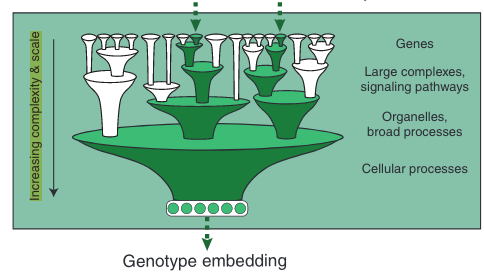
\includegraphics[width=\linewidth]{Figures/drugcell_architecture.png}
    \caption{DrugCell's \cite{kuenzi_predicting_2020} architecture, it is analogous to Reactome but the genes, biological processes and pathways are constructed independently and may not overlap.}
    \label{fig:drugcell}
\end{figure}

We implemented the variant of P-NET informed by Gene Ontology through significantly restructuring the P-NET codebase. The DrugCell code provided by Kuenzi et al. \cite{kuenzi_predicting_2020} was the source of the Gene Ontology gene-pathway hierarchy and was copied into the same directory as the Reactome hierarchy. Then additional functions were created within a new file, $\mathtt{pathway\_encoder.py}$, that utilised a class-based code structure to eliminate redundancy. This was a crucial element of our adaptation of P-NET because it facilitated us to test Reactome and Gene Ontology with a fixed procedure of performance evaluation and hyperparameter optimisation.

\begin{figure}
    \centering
    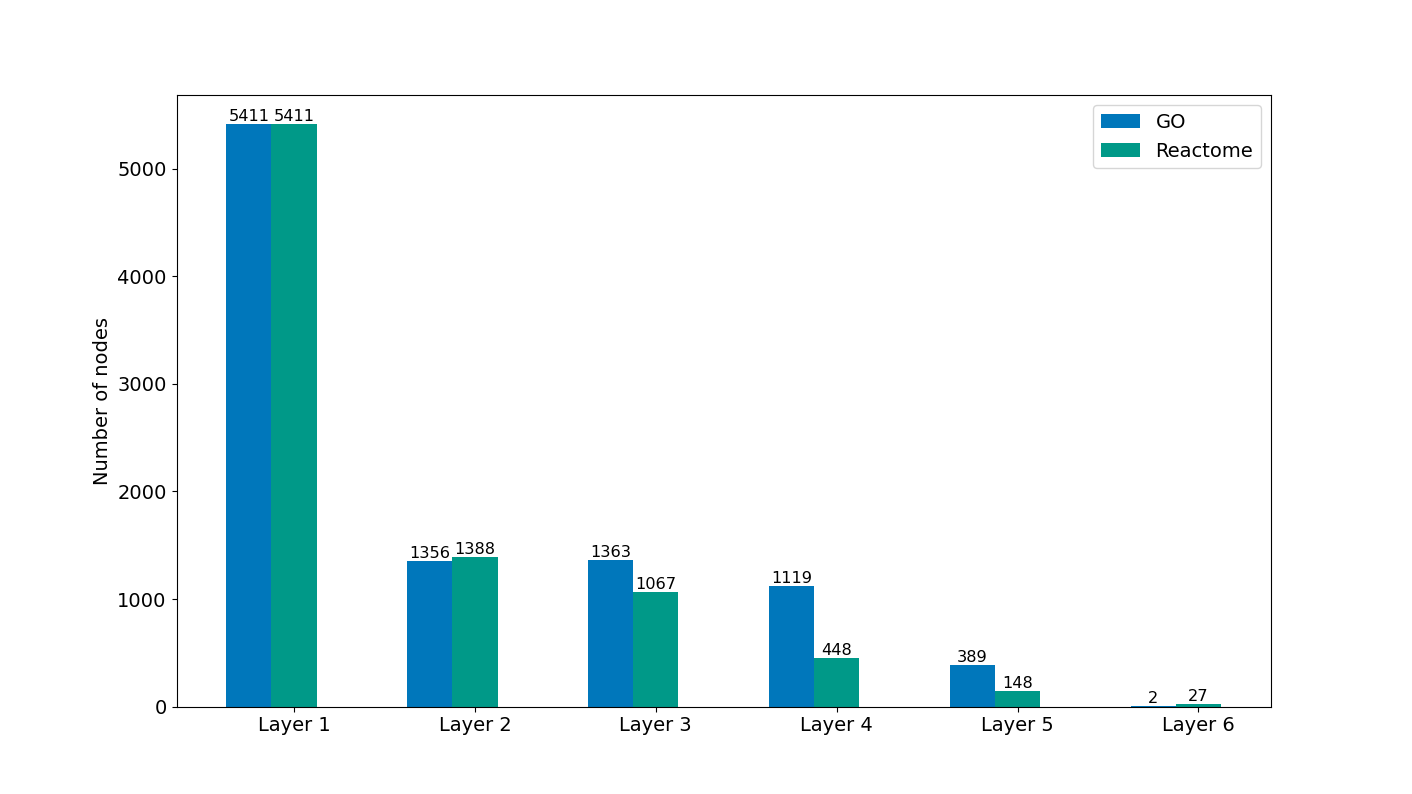
\includegraphics[width=\linewidth]{Figures/layer_node_number.png}
    \caption{The number of neurons contained in each of the 6 network layers, with layer 1 being the input gene layer. The difference in edges in every layer after the first layer is encoded by the different pathways in Gene Ontology and Reactome. Figure inspired by fig. 4.3 in \cite{cosmin_thesis}.}
    \label{fig:nodedist}
\end{figure}

The node distribution in each layer in figure \ref{fig:nodedist} helps to illustrate the advantages of a biologically informed neural network. A dense (fully connected) neural network with the same number of layers and nodes would have $\sim\,3$ million parameters, while a Gene Ontology-informed neural network has $39, 196$ parameters and a Reactome-informed neural network has $37, 144$ parameters. This represents a $\sim 98 \%$ reduction in the number of trainable parameters simply by utilising known biological pathways emanating from genes while preserving the same predictive power by removing impossible connections.

A sparse network is achieved by representing the Gene Ontology or Reactome hierarchies as a mask matrix, $\textbf{M}$ of zeros and ones. Given consecutive layers $l_{1}$ and $l_{2}$ with $n_1$ and $n_2$ neurons respectively, $\textbf{M} \in \{0, 1\}^{n_1 \times n_2}$ is defined by (taken from \cite{cosmin_thesis}) equation \ref{eq:maskmatrix}.

\begin{equation}
    \textbf{M}_{ij} = \left\{ \begin{array}{rcl}
0 & a\,connection\, exists\, in\, the\, Gene\, Ontolgy/Reactome \, hierarchy \\ 1 & no \, connection \, exists \, in \, the \, Gene \, Ontology/Reactome \, hierarchy \end{array}\right.
\label{eq:maskmatrix}
\end{equation}

The mask matrix, $\textbf{M}$ is then multiplied element-wise to the weight matrix, $W \in \R^{n_1 \times n_2}$ to set all connections that do not exist in the Gene Ontology or Reactome hierarchies to $0$. The output of a given layer $l_1$ after an activation function, $f$, will then be \cite{elmarakeby_biologically_2021}, given an arbitrary bias term $\textbf{b}$ equation \ref{eq:layeroutput}.

\begin{equation}
    \textbf{y} = f((\textbf{M} \odot \textbf{W})^T\textbf{x} + \textbf{b})
    \label{eq:layeroutput}
\end{equation}

The original implementation of P-NET \cite{elmarakeby_biologically_2021} used a hyperbolic tangent activation function for all the hidden layers, however, \cite{cosmin_thesis} found that a combination of $ReLU$, $Leaky ReLU$ and $tanh$ demonstrated the best performance. Additional features have been implemented to increase P-NET's robustness against overfitting the training data. Each hidden layer is connected to the next layer in succession, and the final output (example in figure \ref{fig:2}), and the final prediction are calculated as the average of the six resulting outputs. To preserve the independent predictive power of each layer, the outputs of different layers are weighted to increase exponentially with layer number during the loss function computation because of the small number of edges in the final layers \cite{cosmin_thesis}.

\subsection{Loss function}
Each of the 6 layers of the network can be used to predict the radio-sensitivity. To prevent each layer from inheriting features from its parent \cite{cosmin_thesis}, P-NET uses a loss function built by combining the predictions from each of the 6 layers using a vector of loss weights.  We chose the mean squared error as our loss function.
We kept this at the default value for P-NET shown in Table \ref{tab:hyperpars}.
\subsection{Regularization}
Despite the sparse network, the model is still prone to over-fitting. To prevent this we employ $\mathtt{L2}$ regularization. This consists of adding a penalty term to the loss function:
\begin{equation}
    L_{L2} = \lambda \times \sum ||w||^2,
\end{equation}
for all the model weights $w$. This term will push the model towards smaller weights (or thus a simpler model). This term is characterised by the regularisation parameter $\lambda$, too small a value will lead to model overfitting, while too large can cause the weights to diverge to 0. In this case, the model will not predict any variability and instead predict for all outputs the mean of the training data.
\subsection{Early stopping}
We employ early stopping \cite{keras-docs} when training the model to further prevent over-fitting and improve training speed. This prevents very continuing training for many epochs, which while improving the loss function may decrease the validation data loss function. We employ early stopping using a patience of 10, this means that if the validation loss function increases for the patience number of consecutive epochs the training is halted and the weights with the lowest validation loss are used. We tested increasing the patience value but this had negligible effects.
It should be noted that this procedure could potentially lead to a biased validation performance estimate. However, our final performance is quoted on test and not validation data.

\subsection{Cross-validation and hyper-parameter tuning}
Due to the very small available datasets we found the performance of a given model can vary significantly based on the test splitting of the data. In addition, the performance can vary based on the random seeds used in the stochastic minimisation of the loss function. We also found that the performance can depend significantly on model hyper-parameters. If these are tuned to optimise the performance on a particular test splitting of the data this will result in an overly optimistic estimate of the performance when trained on unseen data.

\\ \indent To account for this we have developed a cross-validation procedure. This is used both to tune hyper-parameters and to make an unbiased estimate the model performance with a faithful uncertainty estimate. This procedure allows a fair comparison of different models.

\\ \indent We employ a procedure of nested-random-cross-validation \cite{cross_validate}.
A set of randomly chosen test datasets are selected based on 12\% of the total data. In each case the remaining data is used to tune the model hyper-parameters. For this we use a grid search with random-cross validation. For every hyper-parameter set the data is is partitioned into a validation (12\% of the data) and a training set (the remaining data). The model training is run using the validation set to decide the early stopping of the training and to estimate the performance. This is then repeated a number of times to obtain an estimate of the mean performance and uncertainty for this hyper-parameter set. The hyper-parameter set with the best model performance are then used to train the model, with the performance judged on the test dataset. The distribution of this testing performance give an unbiased estimate of the model performance, with a reliable uncertainty estimate. This procedure is very computationally intensive. For a single model evaluation with nested cross validation $\mathcal{O}(10^4-10^5)$ models are required to be trained. This has been implemented using batch job submission in parallel on the Myriad cluster at UCL \cite{myriad}.

\\ \indent There are a number of hyper-parameters potentially affecting the model performance. For example the learning rate of the gradient descent and learning rate schedule, L2 regularisation parameters, drop-out parameters etc (see more details in the previous section). 
These hyper-parameters can broadly be divided into two classes, those which control the minimisation of the loss function and those which add some terms / modify it to prevent over-fitting. We found most of the hyper-parameters are correlated so focused on two for a optimisation, the learning rate ($\alpha$) and the regularisation parameter ($\lambda$) which are tuned using a grid search.  

\\ \indent Other model hyper-parameters are not formally optimized. To prevent bias these were set to the default P-NET values based on the $\mathtt{scikit-learn}$ and tensor-flow documentation and some initial tests on a single train / validation set. 
The choice of parameters is specified in Table \ref{tab:hyperpars}.
\begin{table}[]
    \centering
    \begin{tabular}{c|c}
       Hyperparameter  &  Value \\ \hline
       Regularisation parameter ($\lambda$) & Optimised - see text \\
       Learning rate ($\alpha$)  & Optimised - see text \\
      batch size  & 50 \\
      Early stopping patience &  10 (reactome) / 30 (Gene Ontology) \\
     Maximum number of epochs &  50 \\
     Optimiser &   Adam \\
     Loss weights &  $[1, 15, 20, 54, 240, 380]$ 
    \end{tabular}
    \caption{The various hyperparameters used in training P-NET for radiation sensitivity.}
    \label{tab:hyperpars}
\end{table}

\\ \indent To asses model performance we compute the $R^2$ score defined as \cite{scikit-learn-docs}:
\begin{equation}
    R^2 = 1-\frac{\sum (y_i - \hat{y}_i)^2}{\sum_i (y_i - \bar{y})^2},
\end{equation}
where $y_i$ the value for data-point $i$, $\hat{y}_i$ is the associated prediction, while $\bar{y}$ is the mean of $y$. This gives a measure of the amount of variance in the outputs explained by the model.
%\input{method}

%---------------------------------------------------------------------


\subsection{Transfer learning}
As previously mentioned in \ref{sec:introduction}, the difficulties in obtaining radio-sensitivity data for human tumour cell lines has provided us with a relatively small dataset of 511 cell lines from the Cleveland dataset. The sparsity P-NET (order $10^5$ trainable parameters) has demonstrated improved performance when compared to fully dense networks (order $10^7$ trainable parameters) for cancer classification, particularly in low data settings by avoiding over-fitting \cite{elmarakeby_biologically_2021}. 

Clearly then, the supplementation of additional information to the Cleveland set may further improve generalisation of the P-NET model. This idea forms the basis of \textit{transfer learning}, where knowledge from related fields can be used to inform machine learning models trained on either field. In the context of this work, our aim is to predict radio-sensitivity, and we hope to use data from drug sensitivity to perform transfer learning. For certain drugs, the underlying cellular processes that cause cell death and proliferation will have similarities to radiation, thereby being more suited for transfer learning. Luckily, databases related to drug response are somewhat more extensive than that of radiation, as discussed in \ref{sec:data}. As seen in Figure \ref{fig:3}, transfer learning assumes that the lowest level features and connections (relations between individual genes) remain somewhat consistent from drug response to radiation response. By training a network on drug response and transferring (and freezing) the lowest layers, the model trained radiation response can be fitted using fewer trainable parameters with hopes of improving performance and reducing over-fitting.

In this project, we built a transfer learning pipeline based on above described hyper-parameter tuning framework. Unfortunately, due to time constraints the outer loop of nested cross-validation was not implemented in the transfer learning pipeline. 

This involved using the hyper-parameter tuning framework to train drug-sensitivity prediction models based, with one model for each of the 10 drugs described in \ref{sec:data}. This can be done in exactly the same way as radio-sensitivity prediction described in \ref{tab:hyperpars}, as the structures of both datasets are represented in the same way mathematically. Best performing hyper-parameters are then saved and optimised drug-sensitivity prediction models are saved. From here, the 3 lowest layers of each model are frozen and transferred to a radio-sensitivity prediction model (also informed by Reactome), setting the weights for the 3 lowest layers. The radio-sensitivity model then goes through hyper-parameter tuning in the same way as in \ref{tab:hyperpars}.
\begin{figure}
    \centering
    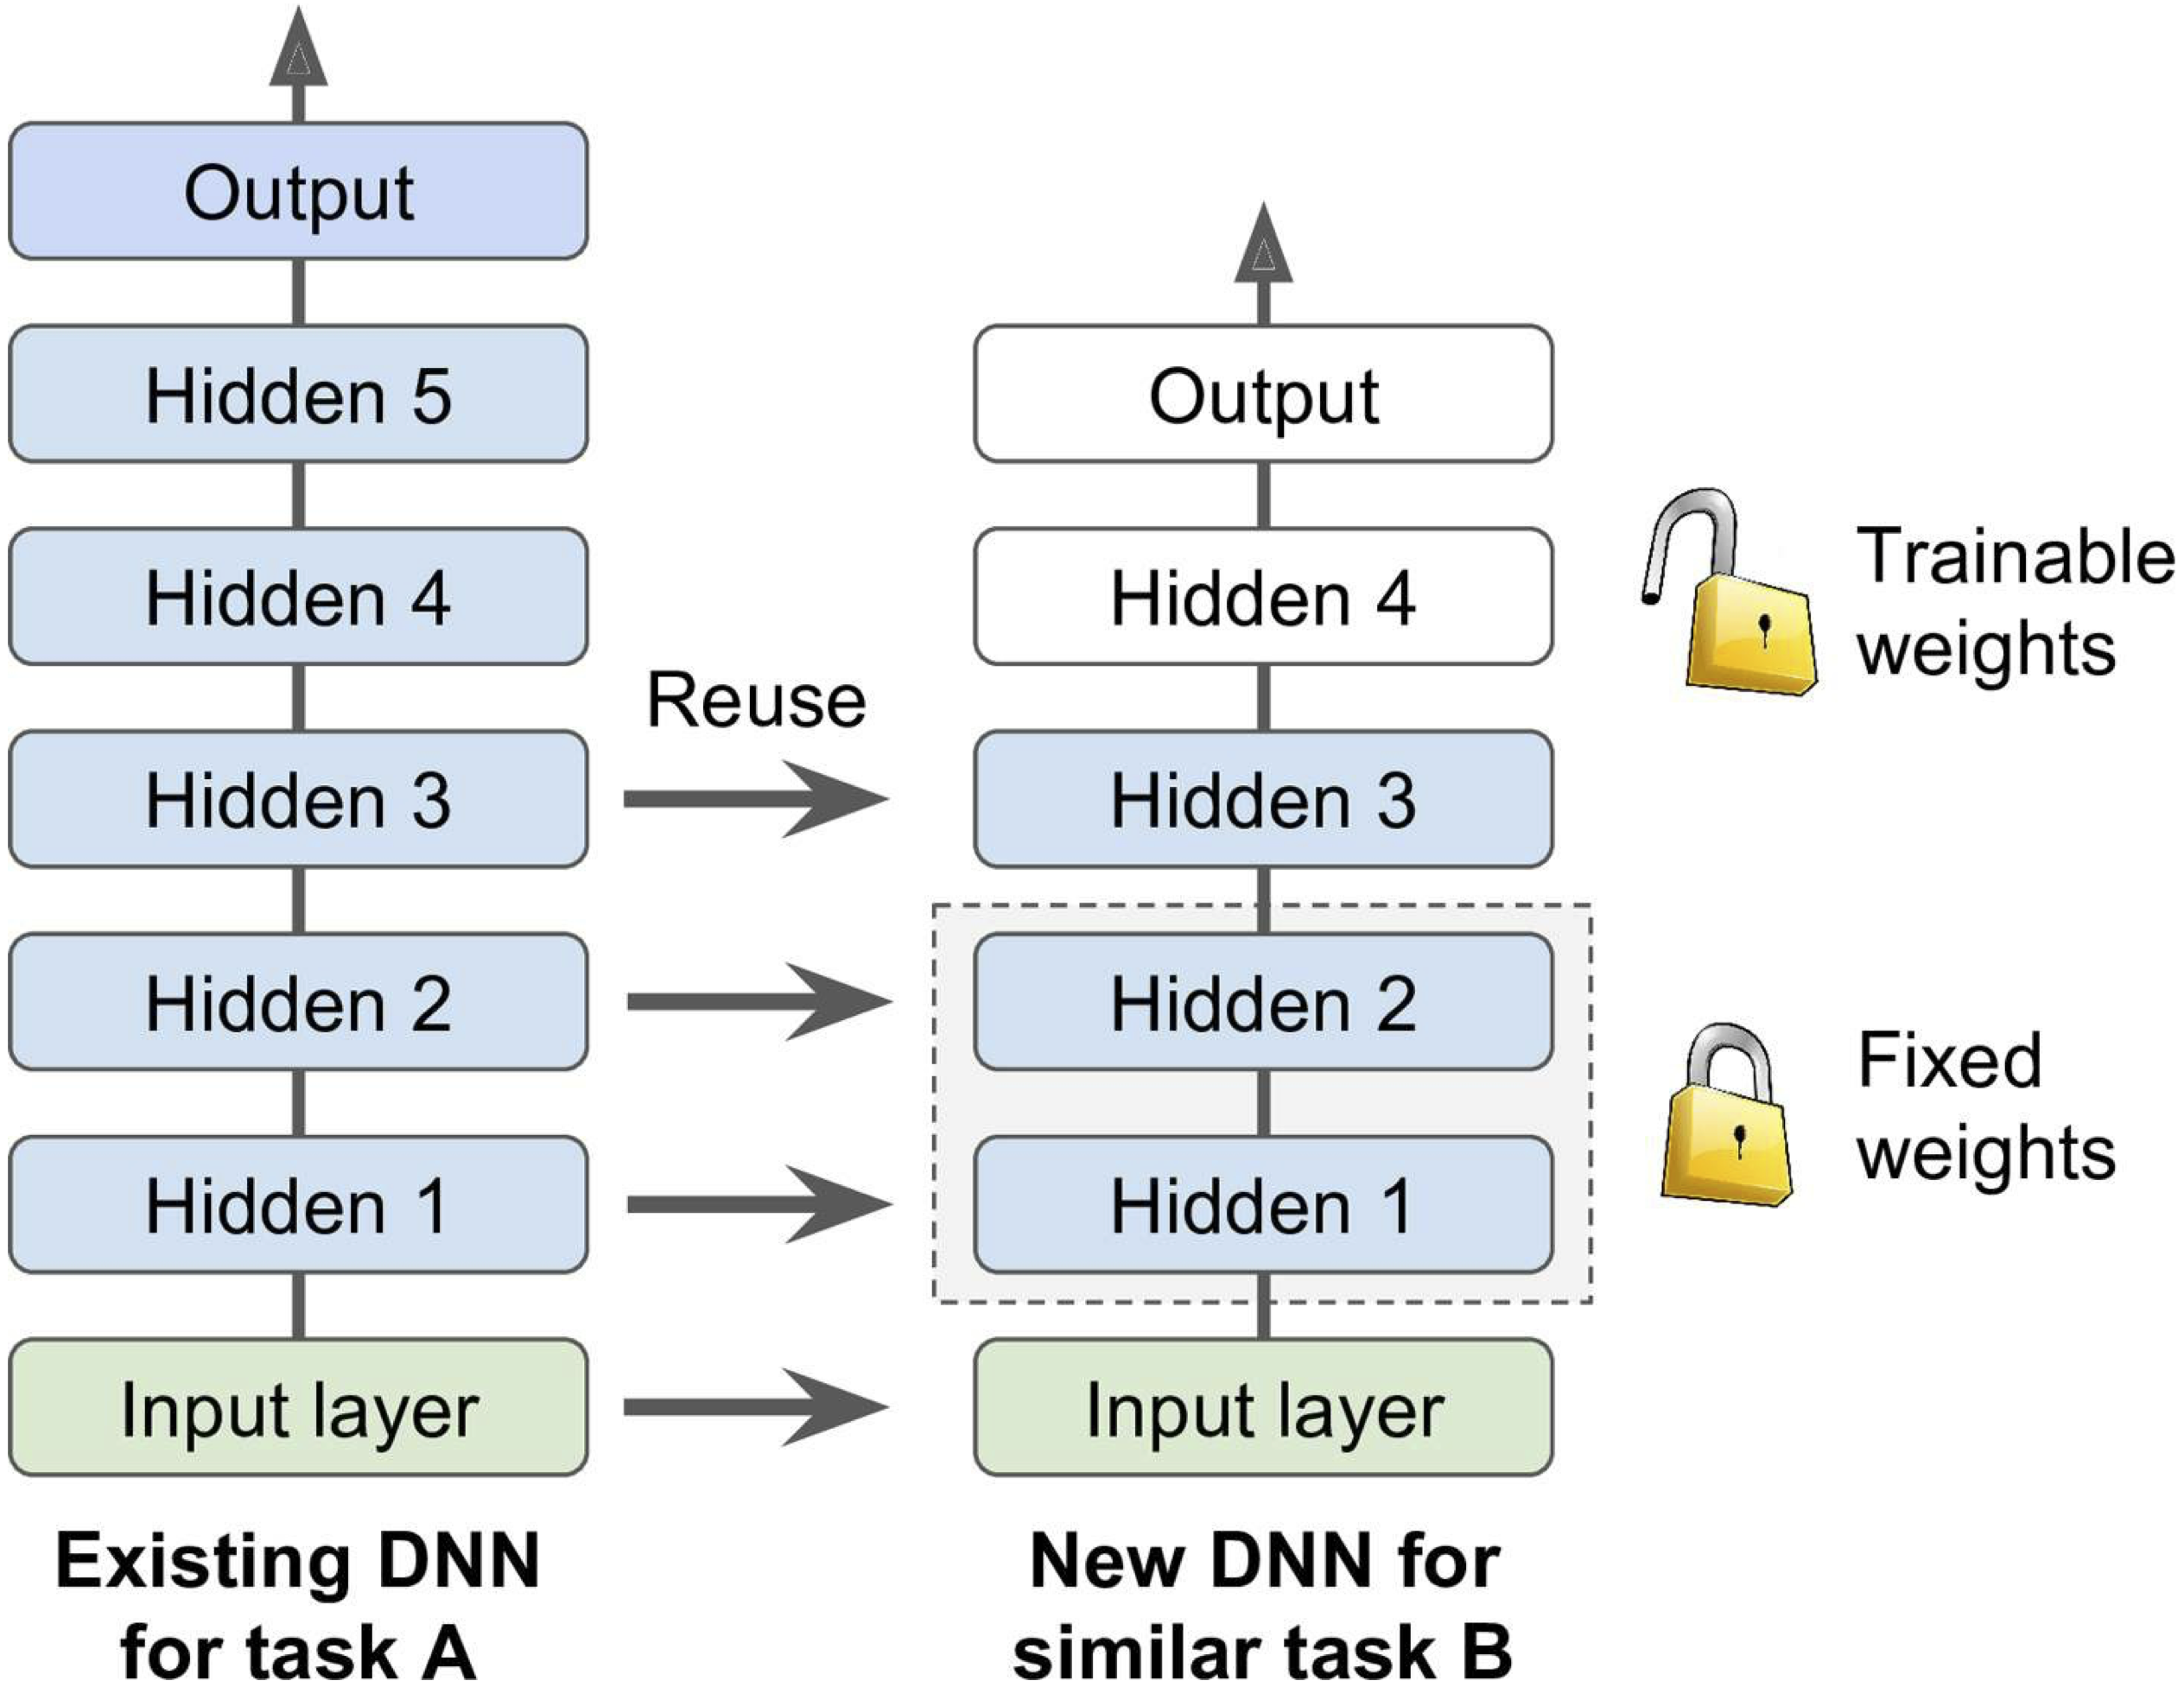
\includegraphics[width=6cm]{Figures/transfer_learning.png}
    \caption{Transfer learning procedure in neural networks \cite{McEwann lecture}}
    \label{fig:3}
\end{figure}

\section{Results}
\label{sec:results}
\\
We use a biologically informed neural network based on P-NET \cite{elmarakeby_biologically_2021} to predict the radiation sensitivity of 511 cell lines. These models are tuned using nested cross validation with a grid search over the main hyperparameters. 
We performed a systematic comparison of P-NET applied to radio-sensitivity predictions using both the Reactome \cite{reactome} and Gene ontology \cite{go_1,go_2} databases and gene expression, copy number variation and mutation data separately. 
\subsection{Reactome network}
First we present results for the model trained using the Reactome network architecture. In \cite{cosmin_thesis}, a similar model was trained using gene expression data. This study used a fix train/test/validation split and hyper-parameter tuning was performed manually. 
We reproduce this study using the same data splitting, but with optimisation of the learning rate and regularisation. 

\\ \indent We observed a large variation in the validation and test performance when changing the random seed used in the batch gradient descent.
This large observed variability is related to the small size of the dataset, along with large number of features. This leads to a large number of local minima in the loss function. 

\\ \indent We optimise the learning rate and regularisation parameter for this dataset. A grid search is performed in the range of $\log{\alpha}\in [-3,-1]$ with 10 steps and $\log{\lambda}\in [-5,-1]$ with 10 steps. For each hyper-parameter set the training is run 10 times.
In Fig. \ref{fig:fix} we show the mean and standard deviation of the validation data $R^2$ distribution for each hyper-parameter set. The best value is found to be $\alpha=10^{-5}$, and $\lambda=10^{-2.1}$. However, there is not a sharp minimum in the distribution, although when the learning rate is decreased below $\sim -2.9$ we observe a sharp drop in performance. The optimal set of hyperparameters leads to average performance of:
\begin{equation}
    R^2 (\mathrm{train})&=60\pm 7 \ \%, \ \       R^2 (\mathrm{validate})&=40\pm 5 \ \%, \ \
    R^2 (\mathrm{test})&=18\pm 5 \ \%. 
\end{equation}
\begin{figure}
    \centering
    \includegraphics[width=0.47\textwidth,page=4]{Figures/fixed_reactome/hyper_scans_validate.pdf}
\includegraphics[width=0.47\textwidth,page=5]{Figures/fixed_reactome/hyper_scans_validate.pdf}

    \caption{Mean (left) and standard deviation (right) of the validation data $R^2$ distribution of P-NET predictions of AUC, obtained with a single train/test/validation split of the data.}
    \label{fig:fix}
\end{figure}
This estimate of the performance on validation or training data is likely biased and was only computed for a comparison with \cite{cosmin_thesis} where a value of 31 \% for test and 42\% for training data was obtained. These values are consistent with what we obtained. It is striking that the performance obtained on the test dataset, not used for the hyper-parameter tuning is much lower than that for the training or validation data. Nested cross-validation is needed to properly asses the uncertainty on this value

An example of the training, test and validation predictions for the optimal hyper-parameters are given in Fig. \ref{example_scatter}. We see that in this case P-NET does a fairly good job at predicting the AUC values, without clear over-fitting. However, we note the performance on test data is less satisfactory and there is a large possible bias in the validation performance.
\begin{figure}
    \centering
    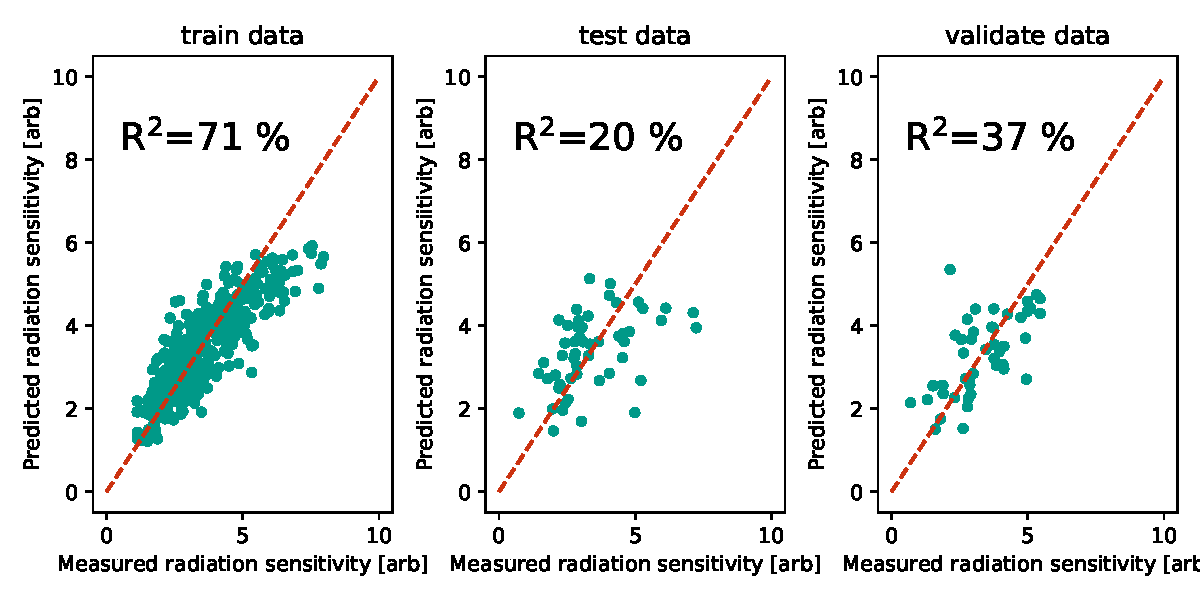
\includegraphics[width=1\textwidth]{Figures/example.pdf}
    \caption{Predicted against measured AUC for P-NET, obtained with a single test/train/validation split of the data. The red line shows prediction = measurement and is included for reference.}
    \label{example_scatter}
\end{figure}

We then repeat this optimisation procedure varying the validation split using cross validation (as described earlier). This represents a single ''outer-loop" of our nested cross validation. In this case the optimal set of hyper-parameters are $\lambda=10^{-1.89}$ and $\alpha=10^{-4.11}$ leading to average performance of:
\begin{equation}
    R^2 (\mathrm{train})&=50\pm 25 \ \%, \ \       R^2 (\mathrm{validate})&=26\pm 13 \ \%, \ \
    R^2 (\mathrm{test})&=8\pm 11\ \%. 
\end{equation}
This performance is notably worse than that obtained on a single validation/ test dataset. In addition, the uncertainties are greatly increased. In the future this algorithm could be improved to consider also the variance in the optimisation, this could produce optimal hyper-parameters which result in both stable performance.
These results demonstrate the bias induced by tuning hyper-parameters to a single dataset and motivated the development of the nested-cross validation procedure described earlier. 

\\ \indent We use the nested cross-validation procedure defined earlier to provide an unbiased estimate of the model performance. 
Across these 10 random test splittings we observe performance of:
\begin{equation}
    R^2=16 \pm 10 \%.
\end{equation}
This indicates that P-NET trained using this data provides a moderately good but very unstable prediction of radiation sensitivity. We note that in most cases the $R^2$ value is above the mean, however for some test datasets we observe a divergence in the training. This results in the model predicting a constant output based on the mean of the training data. Future work will focus on increasing the stability of P-NET to provide this undesirable behaviour.

\\ \indent 
This modest performance motivated the development of the transfer learning algorithm described earlier.
\subsection{Gene Ontology network}
We repeat this procedure of using the Gene Ontology network again using Gene Expression data. We found that a higher early stopping patience value is needed to obtain reasonable results, this is set to 30 for Gene-Ontology. 
The average performance across the 10 test datasets is:
\begin{equation}
    R^2=9\pm 6 \%.
\end{equation}
While this is slightly worse than the performance from Reactome, it is likely some other hyperparameters of the model need to be adjusted for the Gene Ontology network architecture. Alternatively, the poor predictive power could be due to the compression of the gene expression data into only $2$ nodes in layer 6 of P-NET (figure \ref{fig:nodedist}). This could be removing salient features that properly describe the relationship between gene expression and radiation sensitivity. It should be noted that Kuenzi et al.'s DrugCell (\cite{kuenzi_predicting_2020}) implementation uses only $12, 516$ neurons and has $6$ neurons at the output of their Gene Ontology informed neural network to characterise the whole gene ontology. A mismatch in the gene labels in the gene expression data and the Gene Ontology hierarchy could be the cause of there being only two nodes in the final layer.

\subsection{Systematic comparison of data types and architecture}
We repeat the procedure defined above for each data type and for the Gene Ontology as well as Reactome network. The results are shown in Tab. \ref{tab:perf}.  
This represents the first systematic comparison with unbiased performance estimates including uncertainties of a biologically informed neural network applied to radiation prediction using different network architecture and data types.

\\ \indent The baseline Reactome network trained with Gene Expression data provides the best overall performance. CNV, and mutation data alone do not provide a useful predictor of radiation sensitivity.
This could be related to the sparsity of this data where most entries are zero.
However, it remains to be seen whether this data in combination with Gene Expression could improve radio-sensitivity predictions. The framework we have developed in this work allows to easily test this and other possibilities.
\begin{table}[]
    \centering
 \caption{$R^2$ performance of P-NET obtained using nested random cross validation, for different network architecture and data types.}

    \begin{tabular}{c|c|c}
     Data Type    & Network & Test $R^2$ [\%] \\ \hline
 Gene Expression  & Reactome & \ \ $16\pm 10$\\
CNV amplification & Reactome & $-2\pm 5$ \\
CNV deletions & Reactome & $(0 \pm 2)\times 10^{-4}$\\
Mutations & Reactome & $-3\pm4$\\
 Gene Expression  & Gene Ontology& $9\pm 6$\\
CNV amplification & Gene Ontology & $(0.8\pm 0.2)\times 10^{-3}$ \\
CNV deletions & Gene Ontology & $(2\pm 3)\times 10^{-4}$ \\
Mutations & Gene Ontology & ($-1\pm 3)$\%\\
    \end{tabular}
    \label{tab:perf}
\end{table}
\\

\subsection{Transfer learning}

In the same way as described above, both (for drug and radio-sensitivity training) hyper-parameter tuning procedures require a grid search based on only gene expression data. However, this has now been performed over a broader range of $\log{\alpha}\in [-10,-1]$ with 10 steps and $\log{\lambda}\in [-5,-1]$ with 10 steps. Once the optimum for $\alpha$ and $\lambda$ were found, a finer grid search of $\pm 1$ was performed. Naturally, each drug and subsequent radio-sensitivity hyper-parameter tuning procedure led to different sets of hyper-parameters.

\begin{table}[]
    \centering
 \caption{$R^2$ performance of P-NET obtained using transfer learning for a single test set, for the selected sources}
    \begin{tabular}{c|c}
    Source ID    & Test $R^2$ [\%] \\ \hline
     Radiation & $2.1 \pm 8.7$ \\
     Topotecan &  $5.1 \pm 10.6$ \\
     Paclitaxel &  $-5.4 \pm 12.4$ \\
     Irinotecan &  $5.0 \pm 4.8$ \\
     Crizotinib &  $-0.2 \pm 2.4$ \\
     Nvptae684 &  $6.0 \pm 5.4$ \\
     Dovitinib &  $1.084 \pm 6.203$ \\
     Panobinostat &  $-0.28 \pm 8.9$ \\
     LBW242 &  $8.1 \pm 6.6$ \\
     Raf265chir265 &  $6.9 \pm 10.0$ \\
    \end{tabular}
    \label{tab:transfer_perf}
\end{table}
\\

\begin{figure}
    \centering
    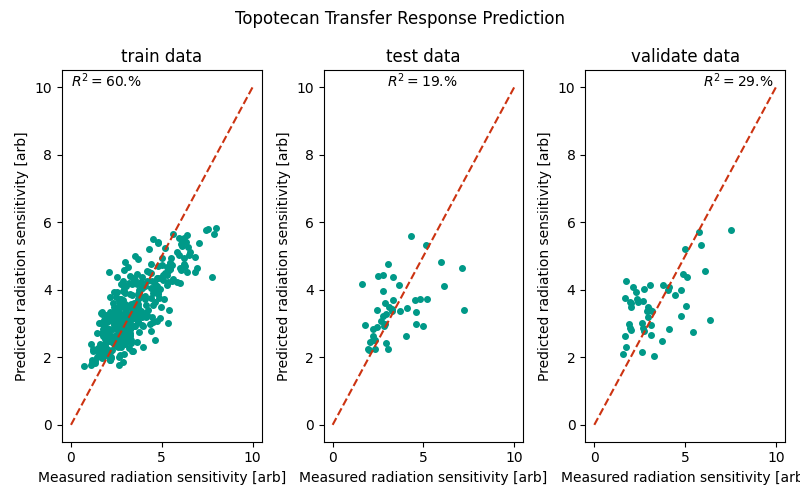
\includegraphics[width=1\textwidth]{Figures/Topotecan_tranfer.png}
    \caption{Predicted against measured radiation response AUC for P-NET using transfer learning from Topotecan, obtained with a single test/train/validation split of the data. The red line shows prediction = measurement and is included for reference.}
    \label{Topotecan_transfer}
\end{figure}

As nested cross-validation was not implemented in the transfer learning, it was not possible to obtain the same type of uncertainty on the transfer learning performance. As such, only a single test set was used, rather than the 10 randomised test sets. However, due to the unstable nature of P-NET, it was still necessary to run the transfer learning pipeline multiple times for the single test set. This was achieved by randomising the train-validation split 50 times to gain an estimate of the performance of transfer learning for the test split. The results of these transfer learning pipelines for the selected drugs are shown in table \ref{tab:transfer_perf}, with the radiation model optimised in the same way as the drug model to establish a fair comparison. An example of the test, train and validation performance of transfer learning used on Topotecan response is shown Figure \ref{Topotecan_transfer}. Although transfer learning may be out performed by the baseline radio-sensitivity prediction for a given train/validation split, table \ref{tab:transfer_perf} indicates that on average, for the chosen test set, transfer learning outperforms the baseline model. This can be confirmed by the fact that the best performing baseline model has $R^2(test) \sim 25\%$ compared to $R^2(test) \sim 20\%$ for transfer learning. A more detailed study of this behaviour is required to understand why this happens. This can be achieved running repeatedly prescribing identical random seeds both pipelines (transfer learning and baseline), and comparing the resulting performances.

It should be noted the above results are almost certainly a biased estimate of the P-NET performance with transfer learning, as only a single test split has been used, and thus the hyper-parameter optimisation is likely to be biased. Regardless, for this test set, it is clear that transfer learning offers promising results. However, a more extensive study is required to verify this claim.

%\input{results}
%---------------------------------------------------------------------

\section{Discussion}
\label{sec:Discussion}

In this report, we presented predictions of cell line radio sensitivity using a biologically informed neural network trained on genetic data. We use an implementation of a BNN based on the P-NET architecture and code base. This has been significantly refactored to allow for a systematic tuning of hyperparameters and nested-random-cross validation run on a high-performance computing cluster and to include the Gene-Ontology network architecture. Furthermore, the refactoring utilises a class-based structure to remove redundant code and to facilitate flexibility in the curated databases, such as Gene Ontology, that inform P-NET.

\\ \indent 
We developed a procedure for tuning the BNN automatically using a procedure of nested cross-validation. We also performed a systematic comparison of different network architectures and multi-omic data types. This showed the model is moderately successful in predicting radio-sensitivity with the best case being the Reactome network trained with Gene Expression data which resulted in an average performance of $R^2=16\pm 10$\%. For Gene Ontology, the best performer is again the Gene Expression data with $R^2=9\pm 6$\%. Although, this is a significant drop in performance when compared to Reactome. Potential explanations include; not conducting the hyperparameter tuning on parameters that the Gene Ontology hierarchy is most sensitive to, this would require a more systematic mapping and testing of all hyperparameters. Secondly, the small number of neurons in the final layer ($2$ in layer $6$ in figure \ref{fig:nodedist}) could be an architectural flaw that could be another explanation. Further study must be conducted on whether the Gene Expression data is being fully matched with the initial genes in the Gene Ontology hierarchy and on the meaning of the ends of the Gene Ontology hierarchy. Too few nodes in layer 6 might be removing too many salient features that are required to explain the relationship between gene expression and radiation sensitivity.

This framework makes it possible to make a statistical comparison of different models, which is critical in the case of omics data with very small datasets and large possibilities of over-fitting or bias in model tuning. \\ \indent

In addition, we have investigated an improvement to this model using transfer learning of drug response data. We obtained promising results showing that the BNN can predict well the drug response in some cases and that this may improve the radio-sensitivity predictions. However, further study is required as the nest cross-validation framework was not applied to the transfer learning pipeline, meaning the results are likely to be biased. Regardless, this demonstrates a proof of concept that radiation responses supplemented by drug response may lead to improvements in the performance of P-NET. This is in line with numerous other studies where similar behaviour has been seen. Furthermore, there is scope for more sophisticated applications of drug data, such as model agnostic meta ("few-shot") learning, where the P-NET model can be adapted to train model parameters that are optimised over multiple tasks by adapting the loss function for best performance overall tasks \cite{MAML}. Another example is multitask learning, which has many possible implementations. In general, this P-NET would require P-NET to learn important features identified across multiple drugs, which can also be based on their mechanism of action and correlation to radiation response \cite{multitask}.


\section{Acknowledgements}
The authors of this report would like to especially express their gratitude to Dr Jamie Dean, Amin Lessan, Felix Crabtree, Cosmin Astefanei, Dr Nikos Nikolaou and the entire UCL radiation lab for their continued support throughout this project. We are grateful for the opportunity to take part in such an interesting which has provided an invaluable learning experience for all the authors.


\printbibliography
%\input{conclusion}
%---------------------------------------------------------------------

\end{document}
